\chapter{Applying the PSO to the FAP}
\label{chpt:psoapplicationFAP}
\section{Introduction}
Particle Swarm Optimization (PSO) as discussed in the overview (see page \pageref{sec:PSO}) is an algorithm that is largely based on the flying behaviour exhibited by a flock of flying birds. Which is why the core of the algorithm is based upon vector math, with new positions and velocities being calculated after each iteration of the algorithm. Thus, a D-dimensional vector represents each particle position and is then simulated flying through the D-dimensional space using the velocity equation (section~\ref{sec:particleVelocity} see page~\pageref{eq:velocityupdate}).

The performance of the Global PSO is benchmarked and outline in the previous chapter. As can be observed from the results presented in the previous chapter, the PSO algorithm produces favourable results on most of the problems it is applied to. Failing to locate the optimum on only a select few problems. 

Most of the problems to which PSO has been applied to, date have been problems where the position of particles have a constant D-dimensional space, which is to formally state \emph{the dimensionality of a particle position in its entirety, is constant}.

This constant dimensionality introduces a intriguing problem if you want to apply the PSO to an inherent multi-dimension problem like the Frequency Assignment Problem (FAP). In this chapter a discussion will be provided on how the PSO was applied to the FAP.

\begin{algorithm}
\label{alg:FAPPSO}
\caption{The FAP PSO algorithm}
\begin{algorithmic}
\STATE $s_n$ = Initialize Swarm $s_n$
\WHILE{Termination criterion not met}
	\STATE EvaluateSwarm($s_n$)
	\STATE UpdateGlobalBest($s_n$)
	\STATE UpdateSwarmMovement($s_n$,$gbest$)
\ENDWHILE
\end{algorithmic}
\end{algorithm}

The first discussion will be on how a particle position is represented in the Frequency Planning domain. This definition of the particle position is important because it plays a central part in
the movement of particles through the Frequency planning domain. After the position definition, a definition will be given on how each position is evaluated as well as a formal definition of the fitness function that the PSO will use in the FAP domain.

Arguably the most important part of the swarm is how the velocity of a particle is calculated and then moving it to a new position in the problem space. The velocity update is important, as it is the primary means by which the algorithm searches problem space.

As was discussed in chapter~\ref{chpt:swarmintelligence} section~\ref{sec:psoonfap} applying the PSO on the FAP introduces a variety of challenges. One of the challenges that were listed is how exactly does one ``fly'' as frequency plan towards another frequency plan. This is an important question that needs to be addressed as the PSO algorithms has no way of searching the problem space by any other means.

To be able to allow the PSO to operate in the FAP space custom velocity functions had to be developed to enable the particles of the swarm to move. A discussion on the various velocity functions that were developed will also be presented in section~\ref{sec:velocityFAP}. 

Developing custom velocity functions for the PSO was simply not enough to achieve good results with the PSO, therefore more innovations needed to be made to improve the solution quality of the PSO. In section~\ref{sec:buildglobalbest} a discussion will be presented on a new mechanism for selecting the global best which enabled the PSO to get better fitness values and therefore direct the swarm more towards better solutions. 

Finally, the chapter will conclude with a section that discusses how the swarm utilizes history to produce better results that enable the PSO to further improve the solution quality.
\section{A Position in the Frequency Planning domain}
In this section a description will be given on what a position is in the Frequency Planning domain. The section will start of by first describing what a Frequency Plan is as well as provide the general structure to represent such a plan. The section will conclude with a discussion on the hard and soft constraints and how it the constraints aid in creating a frequency plan that is suitable for a network.

A Frequency plan, is almost exactly as the name implies. A plan that outlines channels\footnote{See page~\pageref{def:channel} on why frequencies are referred to as channels}(frequency) usage for a wireless network. The benchmark problems that will be used to test the developed PSO, all pertain to cellular phone networks. The benchmarks problems that will be used to test the PSO were presented in chapter~\ref{chpt:fap} section~\ref{sec:FAPBenchmarks}. For Cellular networks, the frequency plan outlines what channel must be allocated to what transceiver.

With this basic definition, the problem is deceptive as one naturally assumes that there are infinite amount channels that can be used or the amount of channels available for assignment is more than the amount of transceivers in the network. 

The reality is, that there are only a finite amount of channels available for cell phone transmissions as was discussed in chapter~\ref{chpt:celltech} and chapter~\ref{chpt:fap}. Hence a regulatory body needs to assign wireless spectrum to cell phone network operators for use in their networks. A regulatory body is needed because, if a network operator just uses any channel it wants, it is bound to interfere with someone else also utilising the same channel.

A network is not assigned the entire wireless spectrum for wireless communication, but rather only a subset is assigned to the network. If one observes the FAP benchmark problems the PSO will be applied upon (see section~\ref{sec:FAPBenchmarks} page~\ref{sec:FAPBenchmarks}) like for instance Siemens1, the allotted spectrum is from channel 16 to channel 90. Which gives the network operator 74 channels to use in its network without considering other constraints. 

Besides the Electro-magnetic constraints that are also applicable here, there are regulatory constraints, like for instance frequencies in the spectrum that are by no means allowed to be used. These frequencies are referred to as globally blocked frequencies and are hard constraints. An in depth discussion on these constraints were given in chapter~\ref{chpt:fap} section~\ref{sec:Interference}.

As discussed in chapter~\ref{chpt:celltech} (page \pageref{chpt:celltech}) and chapter~\ref{chpt:fap} (see page \pageref{chpt:fap}). A Cell phone network is divided into a number of cells, and each cell requires a certain number of transceivers to service its corresponding area. 

The number of transceivers is based on the expected volume of traffic that a particular cell will experience at peak network usage. Some cells might be located in high populous areas, which means the potential traffic that cell might need to handle during peak network usage is very high and thus the cell has more than one transceiver to handle the potential traffic. Whereas with cells that are located in areas that have a low population the potential traffic the cell might experience during peak network usage is low and thus the cell only has one transceiver to handle potential traffic.

Based on the amount of traffic a cell needs to handle the amount of transceivers differs. Thus in a frequency plan all cells do not have the same amount of transceivers otherwise a frequency plan can be modelled as a series of constant D-dimensional vectors. Where the D represents the amount of transceivers. 
~
\begin{figure}[ht]
	\centering
	\setlength \fboxsep{0pt}
	\setlength \fboxrule{0.5pt}
	\fbox{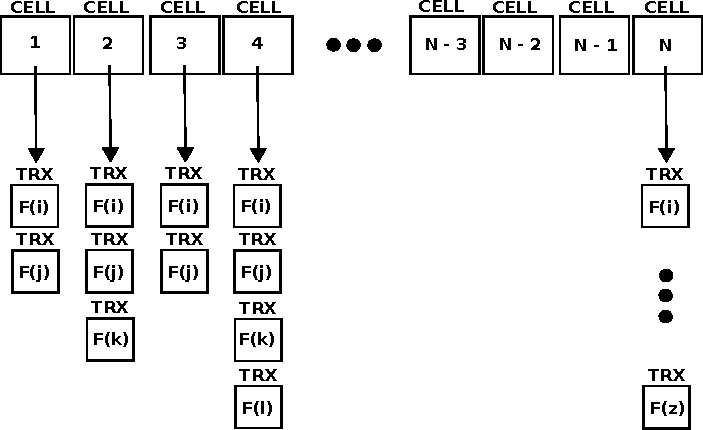
\includegraphics[width=4.8in, height=3.5in]{./pictures/fapPlanDiagram.pdf}}
	\caption{The Structure of a Frequency Plan}
	\label{fig:fapPlan}
\end{figure}
~
As can be seen in figure \ref{fig:fapPlan} a cellular network can have any amount ($N$ in the figure) of cells to attain the desired coverage over the geographical landscape. In the Cost259 benchmarks problems the cellular networks have a large amount of cells that range in numbers from 500 to >1000. 

The most important part of the plan is the actual transceivers within each cell. In figure~\ref{fig:fapPlan} it can clearly be seen, how the amount of transceivers (TRXs) vary from one cell to the next. $F(i)$ is a channel at position $i$ from the available usable spectrum. 

Based on the structure of the plan depicted in figure \ref{fig:fapPlan} there is no concept of which cell interferes with which other cell and if their is indeed interference, how much is inferred as a result. All this information isn't part of the plan. Instead this information, for purpose of this dissertation is supplied by the Cost259 benchmark. 

The interference information is referred to as the interference matrix. A definition of the structure of an interference matrix is given in chapter~\ref{chpt:fap} section~\ref{sec:Interference}. A discussed in the structure definition of an interference matrix each entry references two cells entries Cell A and Cell B. Along with the entry the amount of interference that occurs when Cell B interferes with Cell A is also listed\footnote{Interference occurs based on the electromagnetic constraints as defined in chapter}.

A Frequency Plan is a possible solution to the Frequency Assignment Problem. Therefore in the PSO that was developed each Particle's position in the solution space is represented by a frequency plan. As illustrated in figure~\ref{fig:fapPlan} a frequency plan is just series of cells, where each cell as a set of transceivers. Thus in the PSO algorithm a plan is actually represented as an array of cells. This enables the algorithm to access particular cells in a plan by index as can be observed in listed algorithms~\ref{alg:velocityMethod1,alg:velocityMethod2}. 

Before the particles can actually start to move around in the FAP space, they first need to be assigned positions. In the developed PSO listed in algorithm~\ref{alg:FAPPSO} line 1 the first operation the algorithm executes is to initialize all the particles in the swarm. A particle position in the algorithm is initialized by assigning it a random position. Thus a frequency plan (representing a position) is randomly generated by the algorithm.

The position is purely random in regard that the only considerations that are made by the position generator are that valid channels are assigned to transceivers installed at cells. Thus the generator does not check whether a channel has already been assigned in the current cell or any other considerations. The intended purpose of the generator is just to place a particle in the problem space, not the premature start the optimization process.

Since particles are now able to occupy positions in the FAP space the PSO algorithm is now able to move them around in the problem space. As mentioned previously, moving particles through the frequency plan solution space introduces an interesting problem due to the multi-dimensionality of a plan. A discussion on how particles are moved from one position to another through the solution space will be provided in section \ref{sec:velocityFAP}

In this section a description was given of what the PSO will use as position in the frequency-planning domain. An outline was given on the general structure of what a frequency plan is as well as a definition on how the interference values are retrieved when two cells interfere. In the next section a definition will be given on the fitness function that determines the desirability of a particular particles position or rather the frequency plan its position represents.
\section{The Fitness Function}
In this section a discussion will provided on the fitness function that utilised in all the PSO's that were developed. The fitness function rates the desirability of a particular particles position in the problem space.

As discussed in the previous section, the Cost259 benchmark problems provide an interference matrix that lists the total amount of interference that occurs when a pair of cells interferes. As outlined in the structure definition (see chapter~\ref{chpt:fap} section~\ref{sec:Interference}) each entry in the interference matrix defines a pair of cells that are said to interfere along with two additional values. The first value is referred to as Co-channel interference and is the total amount of interference that will occur on the communication link when the allocated channel of one transceiver is equal to a transceiver in the other cell that is listed in the interference matrix. 

The second value is called adjacent channel interference and it the total amount of interference that will occur on the communication link when the allocated channel of a transceiver in one cell differs by 1 with another channel allocated to the transceiver from the other cell that is listed in the interference matrix.

Particles move towards other particles because the other particles have indicated (through information sharing) that the positions they occupy are very lucrative and thus they have found potential good solutions. The only way particles can know the lucrativeness of the position they occupy is if the position is evaluated with a fitness function. Thus the lucrativeness of a position is actually the fitness value obtained from the fitness function. 

Since a particle position is defined as a frequency plan a procedure is needed that calculates the fitness of a frequency plan. With the FS-FAP the primary concern is to keep interference to a minimum, therefore in the PSO that was developed the fitness value is the total amount of interference generated by all the cells with their allocated frequencies. 

The evaluation procedure goes through each pair of cells defined in the interference matrix where it looks up both cells in the frequency plan. The second cell is said to interfere with the first cell. Therefore each transceiver in the first cell is checked with all the transceivers of the other cell. Depending on whether the frequencies differ from each other, the fitness procedure adds either the co-channel or the adjacent channel interference to a summing variable. This procedure is mathematically defined in chapter 3 see page \pageref{E:costFunction} for the formal equation and the listed algorithm~\ref{alg:fapcost} is the pseudo code of the implement equation used by the PSO. 

As can be seen in algorithm~\ref{alg:fapcost} not all interference values are added to the total amount of interference variable. The Cost259 benchmarks define a Minimum Tolerable interference variable. Which means that if a given interference value is either equal or less than this defined value the interference generated is minute and can be disregarded as it won't have a noticeable impact on the communication link.

In this section an outline of the fitness function the PSO will use to rate the fitness of positions that particles occupy in the solution space after each iteration. In the next section a definition will be given on how particles are moved from one iteration to the next using frequency plans as positions in the solution space.
\section{Velocity Function for Frequency Planning}
\label{sec:velocityFAP}
The Velocity function is arguably the core of the PSO algorithm. It is the procedure by which particles in the swarm move from one point to another point in the solution space. 

The velocity function doesn't blindly move a particle from one point to another but instead, it takes the particle history into account as well as the best particle in the swarm. Therefore, the velocity function is the core means by which
the swarm explores the solution space. A more thorough explanation is provided in section~\ref{sec:particleVelocity} page~\pageref{sec:particleVelocity}.

In this section a discussion will be provided on the development of a velocity function that is suitable for particles to move from one Frequency plan to another. The section will start of with a discussion on the first velocity function that was developed. With each method that will be discussed an outline of the problems associated with it will also be given. 

This section will conclude with the second method that was developed and which is also the primary method the developed PSO uses.

\subsection{Movement in the Frequency Planning domain}
The standard velocity equation works on the basis of vector math. Each particle has a velocity and position, which is represented by a standard mathematical vector. The standard equation alters the direction the particle is moving, to move to a more promising position in the solution space that is in the general direction of the global best particle and a previous personal best position the particle held..

Vector math has standard basic operations defined for adding, subtracting and multiplication. Hence, applying the PSO to problems that are either mathematical functions or problems that map well to the vector domain is a defined process. With regard to the Frequency planning domain an important question needs to be answered. How to move one multi dimension frequency plan to another ?

With any difficult problem it is better to break the problem down into its most basic constructs and then solve each piece individually until the problem as a collective is solved, this technique is also commonly known as Divide and Conquer. This technique was first applied on the nature of a frequency plan.

A frequency plan is a plan that consists of a series of different cells that are in use in the network. The plan specifically specifies the channels each individual transceiver that is installed at a cell must use for communication. Thus a frequency plan can broken up into three important constructs:
\begin{enumerate}
\item A plan is a list of different cells.
\item Each cell in a plan has a list of transceivers that it has installed.
\item Each installed transceiver has a single number allocated to it called the channel. This channel is used for communication.
\end{enumerate}

Now that a frequency plan has been broken up into the constructs it is made up of, the question of how to move one frequency plan to another can be rephrased. How does one move a channel allocated to \emph{transceiver} in a particular \emph{cell} of one frequency plan to another channel of the \emph{same} transceiver and cell in another \emph{different} plan ? An important realisation needs to be note here.

In the PSO at any one time the algorithm is only considering two positions and for the FAP the two positions are frequency plans. Both plans are \emph{identical} except for the specific channels transceivers use. Thus, a cell that exists in the one plan, also exists in another plan. Both the cells have exactly the same amount of transceivers installed, only the channels each individual transceiver uses for communication.

Using this realization, the conclusion can be made that the velocity equation can only work with the channels assigned to transceivers. Therefore, a potential velocity equation mechanism needs to operate on the finest granularity of a frequency plan i.e. the channels.

The principle the first developed velocity method is based upon is for the movement of the swarm to be at a much finer granularity and hence movement is based on channels. Therefore, when a particle needs to move towards a global best particle, the velocity procedure goes into the intricate details of the particle wanting to move and the global best particle. Hence, the procedure goes into each cell defined in the frequency plan represented by the standard particle as well as the global best particle to be able to access each installed transceiver.

To be able to move on frequency plan to another by utilising the standard velocity equation, the equation needs to be broken up into the smaller operations it is made up of. By breaking the equation up into its smaller parts, small operations can be developed that perform the same function as the individual parts. 

The velocity equation in section~\ref{sec:particleVelocity} page~\ref{sec:particleVelocity} can be broken up into the following parts:
\label{lst:velocitybreakup}
\begin{itemize}
\item \textbf{Subtraction} --- $pbest - x_i(t)$ --- (SubtractionResultPbest) and $gbest - x_i(t)$ --- (SubtractionResultGbest)
\item \textbf{Multiplication} --- $c_1\phi_1 * SubtractionResultPbest$ --- (MultiPbestResult) and $c_2\phi_2 * SubtractionResultGbest$ --- (MultiGBestResult)
\item \textbf{Addition} --- $v_i(t) + MultiPbestResult + MultiGBestResult$
\end{itemize}
There are no mathematical constructs that define how two frequency plans are added together or subtracted, let alone multiply. As discussed earlier a frequency plan it is just a series of cells that have channels and these channels are numbers that intern are just integers and there are mathematical constructs that define how two integers should be added, subtracted or multiplied. Both velocity methods that were developed utilise the basic principle that on a fine granularity of a frequency plan you are just working with integers.

\begin{algorithm}
\caption{Velocity method 1}
\label{alg:velocitymethod1}
	\begin{algorithmic}[1]
	\REQUIRE currentParticle
	\REQUIRE globalBestParticle
	\STATE $pbest \leftarrow $currentParticle position
	\STATE $gbest \leftarrow $globalBestParticle position
	\STATE $localCoeff \leftarrow getLocalCoefficient()$
	\STATE $globalCoeff \leftarrow getGlobalCoefficient()$
	\STATE $pBestSubtractResult \leftarrow $Subtract current Particle position from pbest
	\STATE $gBestSubtractResult \leftarrow $Subtract current Particle position from gbest
	\STATE $a \leftarrow $Multiply localCoeff with pBestSubtractResult and a random value
	\STATE $b \leftarrow $Multiply globalCoeff with gBestSubtractResult and a random value
	\IF{first time velocity is calculated for current Particle}
		\STATE $currentParticle.Velocity \leftarrow $Add a and b
	\ELSE
		\STATE $abAdditionResult \leftarrow $Add a and b
		\STATE $inertia \leftarrow getInertia()$
		\STATE $newVelocity \leftarrow $Add abAdditionResult and currentParticle.Velocity
		\STATE $currentParticle.Velocity \leftarrow $Multiply inertia with newVelocity
	\ENDIF
	\STATE $currentParticle.Position \leftarrow $Add currentParticle.Velocity and currentParticle.Position
	\STATE SanatizePosition(currentParticle.Position)
	\end{algorithmic}
\end{algorithm}

The first velocity method is listed in algorithm~\ref{alg:velocitymethod1}. Velocity method 1 works on the principle of moving one cell in a particular frequency plan to the same cell in a different frequency plan. As noted earlier the cells are the \emph{same} but the channels that have been allocated to each transceiver within a cell differs. Thus in velocity method 1 each cell has an array of transceivers. The array of transceivers contains the individual channel numbers that has been allocated to a cell.

Hence, velocity method 1 actually moves one array of transceivers to another array of transceivers. Which is why, if one observes lines 5 -- 17 in algorithm~\ref{alg:velocitymethod1} each particle position gets passed to methods that are named Subtraction, Multiplication and Addition. As discussed in the previous section each position of a particle is in actually a frequency plan. Each of the methods particle positions get passed to will now be briefly explained.

\begin{algorithm}
\caption{Subtract one position from another} (Method 1)
\label{alg:arraySubtract}
\begin{algorithmic}[1]
	\REQUIRE fromPosition
	\REQUIRE toPosition
	\FOR{Each cell $c$ in fromPosition}
		\FOR{Each transceiver $f_{trx}$ in $c$}
			\STATE $t_{trx} \leftarrow$ Get same $f_{trx}$ in toPosition
			\STATE $f_{trx} \leftarrow f_{trx} - t_{trx}$
		\ENDFOR
	\ENDFOR
\end{algorithmic}
\end{algorithm}

The first method that is used to accomplish calculation of the velocity of a frequency plan, is the first basic operation defined in the velocity equation namely Subtraction. As can be observed from algorithm~\ref{alg:arraySubtract}. The particular algorithm expects two positions to be given to it. The position which must be moved from and the another position to where the from position must be move to. As discussed each position is a frequency plan that contains an array of cells, which is why a for-loop is started on line 1 that allows the algorithm to go through each cell that is defined in the frequency plan. Each cell has a number of transceivers which each has an assigned channel. 

To be able to subtract two transceivers from each other, the algorithm needs access to a particular transceiver of cell. The algorithm accomplishes this access by entering another for-loop based on the number of transceivers a cell has as can be observed to occur on line 2. Within this for loop the actual subtraction of transceivers occurs.

The algorithm first obtains the exact same transceiver in the $toPosition$ frequency plan. This operation is quick, as the two plans are identical except for the channels assigned to transceivers for each cell. Thus, the algorithm is able to refer to the cell and specific transceiver in the $toPosition$ plan by the same index it utilizes to access the cell and transceiver in the $fromPosition$.

Once the $toPosition$ plan transceiver channel value has been obtained, the algorithm performs a standard integer subtraction as seen on line 4 of algorithm~\ref{alg:arraySubtract}.
After the subtraction algorithm is completed, a position is returned which is the result of subtracting the fromPosition from the toPosition. Using this result the velocity method 1 algorithm is now ready to apply the next operation of which the velocity update equation consists off, namely multiplication.

\begin{algorithm}
\caption{Multiply position with a value (Method 1)}
\label{alg:arrayMultiply}
\begin{algorithmic}[1]
	\REQUIRE fromPosition
	\REQUIRE value
	\REQUIRE mustRandom
	\FOR{Each cell $c$ in fromPosition}
		\FOR{Each transceiver $trx$ in $c$}
			\IF{must multiply with random number}
				\STATE $trx \leftarrow trx * value * random()$
			\ELSE
				\STATE $trx \leftarrow trx * value$
			\ENDIF
		\ENDFOR
	\ENDFOR
\end{algorithmic}
\end{algorithm}

The multiplication algorithm is where the local Coefficient and the global Coefficient\footnote{Local coefficient is the cognitive component and the global coefficient is the social component. These components are discussed in section~\ref{sec:psointro} page~\pageref{def:socialcomponent}} defined for the PSO get multiplied into a position i.e. frequency plan. As with the subtraction algorithm the multiplication algorithm enters two for loops. The first for loop is to access each cell defined in the frequency plan. The second loop allows the algorithm to access each transceiver within a particular cell. These for-loop can be observed to occur in algorithm~\ref{alg:arrayMultiply} on lines 1 and 2.

Once the algorithm is able to access each individual transceiver and get its assigned channel it is able to perform the multiplication operation. As can be observed in the algorithm on line 3 the algorithm checks whether it needs to multiply the channel with an additional random number besides the $value$ passed to the algorithm. The reason this was done is because of the following cases where multiplication is required in the PSO.

\begin{itemize}
\item The inertia case --- $0.5 * v(t+1)$, where 0.5 is the inertia value and $v(t+1)$ is velocity that has already been calculated for a particular particle $t$. Note, a velocity that has been calculated is still a frequency plan.
\item Standard velocity calculation randomization case --- As can be observed from the velocity equation~\ref{eq:velocityupdate} and also from the multiplication bullet point on page~\pageref{lst:velocitybreakup}, the equation requires that a position must be multiplied with a coefficient $c_1$ or $c_2$ and then a random value $\phi_1$ or $\phi_2$. 
\end{itemize}

Regardless of what case is executed, the actual operation that is performed is integer multiplication, which therefore means even though the inertia and random numbers are decimal the fractional component of result gets discarded. Channels are integers so the loss of the fractional component is warranted as it is of no use.

As per the last bullet point on page~\pageref{lst:velocitybreakup} the last basic operation that occurs in the velocity equation is an integer addition operation. Algorithm~\ref{alg:arrayAdd} is the addition procedure used by velocity method 1 (algorithm~\ref{alg:velocitymethod1}).
\begin{algorithm}
\caption{Add one position to another (Method 1)}
\label{alg:arrayAdd}
\begin{algorithmic}[1]
	\REQUIRE fromPosition
	\REQUIRE toPosition
	\FOR{Each cell $c$ in fromPosition}
		\FOR{Each transceiver $f_{trx}$ in $c$}
			\STATE $t_{trx} \leftarrow$ Get same $f_{trx}$ in toPosition
			\STATE $f_{trx} \leftarrow f_{trx} + t_{trx}$
			\STATE Bound($t_{trx}$)
		\ENDFOR
	\ENDFOR
\end{algorithmic}
\end{algorithm}

In the addition algorithm as with multiplication and subtraction, two for-loops are started as can be observed on lines 1 -- 2. The algorithm first start iterating through all the cells present in the fromPosition frequency plan and then within the cell for-loop starts another for-loop which iterates through each cells transceivers. Inside the transceiver for-loop the algorithm actually performs the addition of two channels.

Two channels are added based on integer addition. Once the fromPosition cell transceiver is accessed, the algorithm retrieves the exact transceiver and cell in the toPosition in order to get its allocated channel value. After both values have been retrieved the algorithm performs the addition as can be observed on line 4 of algorithm~\ref{alg:arrayAdd}.

The addition operation is the last operation that occurs in the velocity equation and is also the only operation that occurs when the resultant velocity is applied to the current position of a particle as in equation~\ref{eq:positionupdate}. Since the addition operation is also used in the final position update of the particle, the addition algorithm has as its last operation in the transceiver loop a bound operation. 

The purpose of the bound operation is to the keep channels within valid value ranges. More on keeping the channel values bounded will be discussed in the next section.
\subsection{Keeping frequencies bounded}
In the previous section a discussion was presented on the first velocity method that was developed. The velocity method is important as it calculates the direction and next position of a particle in the problem space, where the problem space is the FAP and a position of a particle is a possible frequency plan. With the velocity method defined the swarm is now able to move around in the problem space, but this alone is not enough. The swarm has no concept of the constraints\footnote{Constraints in the FAP are discussed in chapter~\ref{chpt:fap}} that are imposed inherently on the domain as well as the network for which a frequency plan is being created for.
\begin{algorithm}
\caption{BoundValue method}
\label{alg:boundvalue}
\begin{algorithmic}[1]
	\REQUIRE Position
	\FOR{Each cell $c_i$ in Position}
		\FOR{Each transceiver $trx_j$ in $c_i$}
			\STATE $trx_j = \left|trx_j\right|$
			\IF{$trx_j \geq maxChannelValue$}
				\STATE $trx_j = minChannelValue + (\text{$trx_j$ mod $maxChannelValue$})$
			\ELSE 
				\IF{$trx_j \leq minChannelValue$}
					\STATE BoundValue($trx_j + minChannelValue$)
				\ENDIF
			\ENDIF
		\ENDFOR
	\ENDFOR
\end{algorithmic}
\end{algorithm}
The constraints that are imposed are usually some part of the spectrum is under no circumstance allowed to be used anywhere in the network, which as discussed in chapter~\ref{chpt:fap} is known as Globally Blocked Channels. Some channels are not allowed to be used only in certain parts of the network, these channels are known as Locally Blocked Channels. Then of course the swarm also needs to take into account the electromagnetic constraints\footnote{Discussed in chapter~\ref{chpt:fap} section~\ref{sec:Interference}}.

Therefore, the velocity function used by the PSO needs to be altered to make the swarm in some sense more aware of the domain it is operating in and hence keep the particle positions bounded within the allowable search space. By not bounding particle positions in the FAP problem space, transceivers of some cells might get assigned a channel that is not allowed or not even allocated to the network. The PSO will accept this assignment since the fitness function operates on the assumption that under no circumstance will these invalid channels be assigned and thus does not penalize invalid assignments.

Thus to keep assigned channel values to transceivers in the allocated spectrum of the network a boundary check needs to added to the velocity method. The purpose of the boundary check is to validate all assignments in a position i.e. frequency plan a particle currently occupies and if any assignments violate the defined boundary constraints then to take the violating value and modify is to be in the acceptable value range.

The boundary check that is used by velocity method 1 operates on the bases that for any range of values there are a defined lower bound (a minimum value) and higher bound (a maximum value). The channel boundary check is only applied when one of the following conditions are met after the calculated velocity has been applied to the current position:
\begin{itemize}
\item If a channel allocated to a transceiver is above the maximum allowable channel (higher bound) given to the network. 
\item If a channel allocated to a transceiver is below the minimum allowable channel (lower bound) given to the network.
\end{itemize}

As can be seen on line 5 of algorithm~\ref{alg:boundvalue} a mod operation is applied to the value to bring it within the allowable range. The integer mod operation is similar to integer division the only difference is in the result that is produce. Division gives the result of two numbers being divided. Mod gives the remainder of two numbers being divided. If two numbers divide perfectly into one another there won't be any remainder, if the numbers do not divide perfectly into one another there will be a remainder. 
\begin{align}
	10 mod 50 =& 10 \\
	60 mod 50 =& 10 \\
	50 mod 50 =& 0 \\
	100 mod 50 =& 0 \\
	35 mod 50 =& 35 
\end{align}

As can be seen in the above example mod operations, any value that gets modded will be kept in the range $[0,50]$. With regard to channels, the following occurs. If for instance, the maximum allowable channel is 50, and the transceiver has a channel value (after velocity) is 56. The 56 value gets modded with 50 to produce a value of 6. This modded value is then added to the minimum allowable channel. In essence, the value is wrapped around to always be within acceptable range. 

The difficult case is when the channel value is lower that the minimum channel given to the network. This is because modding the channel value has no effect. For example, if the lowest allowable channel is 20 and the transceiver value after movement is 15.
Modding the transceiver value of 15 with 20 has no effect. To solve this, the following options were considered.

\begin{enumerate}
\item First subtract the lower value from the minimum allowable channel. Then add the result to the minimum allowable channel. The resultant value is checked again whether it oversteps the bounds of the maximum allowable channel and bounded accordingly.
\item Add the lower value to the minimum allowable channel. The resultant value is checked whether it oversteps the bounds of the maximum allowable channel and bounded accordingly.
\item Repeatedly subtract the lower value from the maximum allowable channel until the resultant channel is within the acceptable channel range.
\end{enumerate}

An important notion to consider is that based on the velocity equation it is entirely in the realm of possibility that a channel value after movement might contain a negative value. As can be seen on line 3 of algorithm~\ref{alg:boundvalue} the algorithm solves this problem by first taking the absolute value of negative channel value. The boundary check then treats the now positive channel value, as a normal value that needs to be bounded.

In this section a discussion was presented on how the developed PSO keeps all frequency plans that represent the positions of the swarm valid. The problem that occurs to due applying the velocity equation was discussed and an algorithm was presented that solves this problem. In the next section a discussion will be presented on why it is better to use channel index values rather than actual channel values for frequency plans. 
\subsection{Using indices instead of frequencies}
\label{sec:velocityFAP2}
As discussed in section~\ref{sec:velocityFAP} and as can be observed from algorithm~\ref{alg:velocitymethod1} the first velocity method that was developed for the PSO worked with raw channel values. This is not ideal since upon closer inspection the channel range the swarm used to move around was indeed incorrect. The bound value algorithm only keeps channels within a minimum and maximum allowable channel range, but Globally Blocked Channels and Locally Blocked Channels can be in between this minimum and maximum channel range. 

Thus with velocity method 1 and the PSO using raw channel values, the swarm increasingly moved towards allocating these blocked channels to transceivers since the fitness function does not penalize the use of blocked or invalid channel values. This is due in part because these values are under no circumstances allowed to be used and thus the fitness function is not designed to check for these values explicitly to impose a penalty.

Frequency plans that utilize these blocked channels are invalid and cannot be used. If a network were to use a plan that uses blocked channels it can cause unexpected interference to other services and the network can be fined by the governing body who controls the spectrum. A bare minimum requirement then is that the PSO must generate valid frequency plans and hence swarm particles can only occupy valid positions. The following options were presented to solve the problem of particles moving towards invalid positions and hence having invalid frequency plans:
\begin{enumerate}
\item Modify the fitness function to penalize a frequency plan if it uses any Globally Blocked Channels or Locally Blocked Channels.
\item Instead of letting the swarm work with raw channel values, rather let the swarm work with indices of an array. The array indices values indicate positions in a array that has been pre-filled with only \emph{valid} channels. Thus the swarm then moves around in a range from 0 to $F$, where $F$ is the size of the channel array.
\end{enumerate}

With the first solution, the fitness function will have to be modified to levy a penalty if a prohibited frequency value is used. The first proposed solution was disregarded because it introduces complexity which can be completely avoided with the second proposed solution.

Where as with the second solution the fitness function will not have to be modified and the boundary check is simplified since there is no need to check for a lower bound any more. The boundary check only now has to check for negative index values and if the higher bound is violated which is now, the size of the array.
\begin{algorithm}
\caption{Velocity method 2}
\label{alg:velocitymethod2}
\begin{algorithmic}[1]
	\REQUIRE currentParticle
	\REQUIRE globalBestParticle
	\STATE $currPos \leftarrow$ currentParticle position
	\STATE $pbestPos \leftarrow$ currentParticle best position
	\STATE $gbestPos \leftarrow$ global best particle position
	\FOR{Each cell $c$ in $currPos$}
		\STATE $c_{pbestPos} \leftarrow $ Same cell in $pbestPos$
		\STATE $c_{gbestPos} \leftarrow $ Same cell in $gbestPos$
		\STATE $movedIndices \leftarrow $MoveIndices($c_{pbestPos},c,c_{gbestPos}$)
		\IF{First time velocity is calculated}
			\STATE ApplyVelocity(c,movedIndices)
		\ELSE
			\STATE $newVelocity \leftarrow CalculateIndexVelocity(currPos.velocity,movedIndices)$
			\STATE ApplyVelocity(c,newVelocity)
		\ENDIF
	\ENDFOR
	\STATE SanatizePosition(currPos)
\end{algorithmic}
\end{algorithm}
Using the notion of rather working with index values than with raw channel values a second velocity method was developed. Algorithm~\ref{alg:velocitymethod2} is where the pseudo code is presented for the second velocity method. The second velocity method differs from velocity method 1 due to it being designed to only work with indices of an array.

The velocity method 2 also differs from method 1 due to manner it applies the velocity equation. Velocity method 1 applies the velocity equation in stages. Each stage is applied to the entire position i.e. frequency plan before applying the next stage. Where as with velocity method 2 the algorithm first enters a for-loop as on line 6. Within this for-loop the algorithm obtains the current cell, the cell stored in its previous best-held position $pbestPos$ and the same cell stored in the global best position $gbestPos$.

Once all the corrects cells have been obtained the algorithm calls a method named \emph{MoveIndices} which is presented in algorithm~\ref{alg:moveindices} as passed all the obtained cells to the method.
\begin{algorithm}
\caption {MoveIndices}
\label{alg:moveindices}
\begin{algorithmic}[1]
	\REQUIRE pbestCell
	\REQUIRE currCell
	\REQUIRE gbestCell
	\FOR{Each $trx_i$ in currCell}
		\STATE $pbestTRX_i$ = Get $trx_i$ in pbestCell
		\STATE $gbestTRX_i$ = Get $trx_i$ in gbestCell
		\STATE $r1 \leftarrow$ Random double number
		\STATE $r2 \leftarrow$ Random double number
		\STATE $localCoeff \leftarrow getLocalCoefficient()$
		\STATE $globalCoeff \leftarrow getGlobalCoefficient()$
		\STATE $a \leftarrow localCoef * r1 * (pbestTRX_i - trx_i)$
		\STATE $b \leftarrow globalCoef * r2 * (pbestTRX_i - gbestTRX_i)$
		\STATE $trx_i \leftarrow a + b$
	\ENDFOR
\end{algorithmic}
\end{algorithm}

In the MoveIndices algorithm three cells are passed to it. The current cell of the velocity algorithm is moving, the same cell that is stored in the previous best held position of the particle and also the same cell in the global best position. The algorithm starts of by iterating through all the transceivers installed at the current cell as can be seen on line 1 of algorithm~\ref{alg:moveindices}. On lines 2 -- 3 the algorithm obtains the channel values from the \emph{pbestCell} and \emph{gbestCell}.

After the MoveIndices algorithm has obtained the channel values it is ready to apply the velocity equation. As can be seen on lines 8 -- 10 the algorithm applies the standard velocity equation~\ref{eq:velocityupdate} formulated in chapter~\ref{chpt:swarm}. 

Once the MoveIndices algorithm has complete, the currCell variable now stores the calculated velocity. Algorithm~\ref{alg:velocitymethod2} uses the return calculated velocity to update the cell position of the current particle. The algorithm accomplishes this by first determining whether the particle has had a previously calculated velocity. If it is the first time velocity has been calculated the algorithm just applies the velocity by using algorithm~\ref{alg:applyvelocity}. 

\begin{algorithm}
\caption{ApplyVelocity}
\label{alg:applyvelocity}
\begin{algorithmic}[1]
	\REQUIRE currPos
	\REQUIRE velocity
	\FOR{Each index $c_i$ in currPos}
		\STATE $c_i \leftarrow c_i + velocity_i$
	\ENDFOR
\end{algorithmic}
\end{algorithm}

Otherwise if the particle does have a current velocity, the algorithm first executes algorithm~\ref{alg:calcindexvelocity} as can be observed to occur on line 11 of algorithm~\ref{alg:velocitymethod2} before applying the calculated velocity with algorithm~\ref{alg:applyvelocity}. Velocity method 2 first executes algorithm~\ref{alg:calcindexvelocity} to apply the concept of inertia~\footnote{Inertia is discussed in chapter~\ref{chpt:swarm} in the sub section titled ``Inertia weight'' of section~\ref{sec:psocharacteristics}.}.

\begin{algorithm}
\caption{CalculateIndexVelocity}
\label{alg:calcindexvelocity}
\begin{algorithmic}[1]
	\REQUIRE currVelocity
	\REQUIRE newVelocity
	\FOR{Each value $v_i$ in currVelocity}
		\STATE $inertia \leftarrow getInertia()$
		\STATE $v_i \leftarrow v_i + (inertia * newVelocity_i)$
	\ENDFOR
\end{algorithmic}
\end{algorithm}

As can be observed in algorithm~\ref{alg:calcindexvelocity} the CalculateIndexVelocity method loops the current velocity. Within the loop the algorithm retrieves the inertia value that needs to be applied after which the inertia value is multiplied with the newVelocity value.

After the CalculateIndexVelocity algorithm has finished executing, the concept of inertia has been applied to the velocity. Velocity method 2 therefore applies the velocity using the ApplyVelocity method listed in algorithm~\ref{alg:applyvelocity} to the current cell found in the particle position to move it in order to obtained a new position.

The observant reader might have noticed that in all the velocity algorithm presented and associated algorithms the procedures operate and store the result in the current particle position that is currently being work on, naturally one might think that this overwrites the position information currently that position. In the developed PSO algorithm when velocity is calculated the respective velocity methods operates on clones of the original position. The original position is only is only used once the velocity has been calculated and the particle must be actually moved.

Another important note, is that if one analyse velocity method one, the switch to using index values instead of raw channels does not effect the methods operation. Since the method only requires explicit knowledge on the data to operates on in the BoundValue algorithm, the algorithm is able to still calculate velocity. 

It is up to the algorithm designer, to update the boundvalue method to rather use the array index bounds than the raw lower and higher bounds of the channels. The BoundValue algorithm needs to be updated since it the primary means by which velocity method 1 ensures valid positions.

Both the velocity method that are utilized by the developed FAP PSO algorithm have now been explained with corresponding pseudo code. The only parts of both velocity equations that have not been discussed in the SanatizePosition methods that gets called right at the end of each velocity method. The SanatizeMethod will be listed and discussed in section~\ref{sec:keepinghistory}.

In this section velocity method 2 was discussed and also why the developed PSO was modified to rather operate on channel index values rather than channel values. All the algorithms that enable to algorithm to accomplish particle movement with indices were also discussed. The PSO is hence able to move the particles in the FAP using two different methods, but for a particle to be moved it needs a personal best and most importantly, a global best to move towards. In the next section a discussion is presented on how the developed PSO algorithm differs from the standard PSO with regard to selecting a global best.
\section{Building a Global Best}
\label{sec:buildglobalbest}
Selection of the global best particle by the swarm is a very important procedure. After the swarm has determined which particle has achieved the best position, the swarm enters the velocity function phase. 

As discussed in the velocity function section and in the Particle Velocity section on page ~\pageref{sec:particleVelocity} each particle position is then modified to move in the general direction of the global best and personal best position. Therefore the global best acts as a beacon for the rest of the swarm in the solution space to indicate where good solutions seem to be for the rest of the swarm.

\begin{algorithm}
\caption{Standard Gbest selection in FAP PSO}
\label{alg:psogbestselection}
\begin{algorithmic}[1]
\REQUIRE swarm
\REQUIRE gbest
\STATE $gbestCost$ = Evaluate(gbest)
\FOR{Each particle $p_i$ in swarm}
	\STATE $cost$ = Evaluate($p_i$)
	\IF{$cost \leq gbestCost$}
		\STATE $gbestCost = cost$
		\STATE gbest = $p_i$
	\ENDIF
\ENDFOR
\RETURN gbest
\end{algorithmic}
\end{algorithm}

Initially the FAP PSO algorithm used the standard method for selecting the global best particle from the swarm and did not differ at all from the traditional global PSO algorithm. The standard global best selection is listed in algorithm~\ref{alg:psogbestselection}. 

As can be observed on lines 2 -- 8 the FAP PSO algorithm loops through all the particle in the swarm and apply the fitness function to evaluate the fitness of the particles position. The fitness value is also referred to as the cost. In the FAP PSO the cost or fitness value of a particle position is the amount of interference the frequency plan that represents the particles position, generates.

A low cost value is preferred of a high cost value, since a low cost value indicates low interference. On lines 4--6 of algorithm~\ref{alg:psogbestselection} the FAP PSO algorithm determines whether the current particle position has a lower cost value than the current global best particle position.

If the current particle position evaluates to a lower cost value than the stored global best, the algorithm replaces the current global best with the current particle being evaluated, which in the algorithm is $p_i$.

Selecting the global best by evaluating the position as a whole seems to be a natural fit. As outlined in the critical evaluation of each algorithm presented in chapter~\ref{chpt:heuristic} and chapter~\ref{chpt:swarm} some of the algorithms had a problem with regard to some cells or even transceivers overshadowing better cells or transceivers.

For this dissertation, overshadowing is a term that describes a scenario where a bad value of one part of the frequency plan is so large, that it causes other smaller values within the frequency plan to not be considered. 

As per the following example a few in a frequency plan might have the worst possible channels assigned to their respective transceivers, where as some of the other cells in the frequency plan might have the best possible channels assigned to their transceivers. Now the few cells with the worst channels generate lots of interference, where as the cells with the best channels generate almost nothing.

When the example frequency plan gets evaluated, the bad cells push up the cost value. The high cost value of the frequency plan makes that the PSO algorithm disregard the whole plan. By discarding the whole plan the FAP PSO algorithm loses that knowledge gained on the few cells that had their best channels assigned to their respective transceivers.

Therefore, in the traditional method of selecting the global best, a particle is actually selected as the swarm best because it contains less overshadowing cells or transceivers. Hence potential good channel assignments get lost.

The FAP PSO therefore needed to exploit the knowledge that the fitness function exposes much more thoroughly. The information exposed by the fitness function allows one to see what effects certain channel assignments have on the interference of the cell when assigned to the individual transceivers. Therefore, to make better use of this fitness information two methods were developed for the FAP PSO, each one being finer grained than the other.

\begin{enumerate}
\item Besides the particle storing its fitness or cost, the particle also needed to store the interference generated by an entire cell due to the channels allocated to its installed transceivers.
\item Besides the particle also storing the total fitness, the particle also needed to store the interference generated by a channel allocated to a particular transceiver of a cell.
\end{enumerate}

With both these methods, the global best selection scheme needs to be changed to allow the swarm to take advantage of this newly exposed information. As discussed, initially the FAP PSO used the standard global best selection scheme listed in algorithm~\ref{alg:psogbestselection}, but now with these new methods, a global best position is not selected any more but instead a global best is built.

Before the FAP PSO is able to build a global best, the way a particle stores its evaluated fitness needs to change. For the standard global selection scheme, the particle only needs to store one fitness value that is a result of evaluating the whole frequency plan. To be able to build a global best as described above, the fitness value cannot simply be one lump sum representing interference. Instead in the FAP PSO algorithm the interference generated by a each and every transceiver is stored.

Thus the FAP PSO is able to know the performance of each an every single channel allocated to a particular transceiver and also compare the allocation to other similar transceivers in other frequency plans.

\begin{algorithm}
\caption{Building Global Best with Cells}
\label{alg:gbestcells}
\begin{algorithmic}[1]
\REQUIRE gbest
\REQUIRE swarm
\FOR{Each particle $p_i$ in swarm}
	\FOR{Each cell $c_j$ in $p_i$}
		\STATE $gbestcell_j$ = Get cell $c_j$ in gbest
		\STATE $cellCost$ = Get total interference for cell $c_j$
		\STATE $gbestCellCost$ = Get total interference for cell $gbestcell_j$
		\IF{$cellCost \leq gbestCellCost$}
			\STATE $gbestcell_j$ = $c_j$
		\ENDIF
	\ENDFOR
\ENDFOR
\end{algorithmic}
\end{algorithm}

\begin{algorithm}
\caption{Building Global Best with transceivers}
\label{alg:gbesttrx}
\begin{algorithmic}[1]
\REQUIRE gbest
\REQUIRE swarm
\FOR{Each particle $p_i$ in swarm}
	\FOR{Each cell $c_j$ in $p_i$}
		\FOR{Each transceiver $trx_k$ in $c_j$}
			\STATE $gbestTrx_k$ = Get $trx_k$ in $c_j$ in gbest
			\STATE $trxCost$ = Get total interference for $trx_k$
			\STATE $gbestTrxCost$ = Get total interference for cell $gbestTrx_j$
			\IF{$trxCost \leq gbestTrxCost$}
				\STATE $gbestTrx_k$ = $trx_k$
			\ENDIF
		\ENDFOR
	\ENDFOR
\ENDFOR
\end{algorithmic}
\end{algorithm}
Each global best scheme developed for the FAP PSO is more finely grained than the other with regard to what the scheme uses to build a gbest. The listed algorithm~\ref{alg:gbestcells} uses interference information of cells to build a gbest. Where as, the listed algorithm~\ref{alg:gbesttrx} utilizes the interference generated by each and every transceiver installed at a cell to build a gbest. Since each cell has transceivers, the second algorithm is therefore more finer grained than algorithm~\ref{alg:gbestcells}.

Each algorithm will now be discussed since the difference between them is subtle. Algorithm~\ref{alg:gbestcells} was the first global best building scheme which was developed and thus will be discussed first. The algorithm starts of on line 1 by iterating through all the particles in the swarm. For each particle the algorithm enters another loop as can be observed on line 2 of algorithm~\ref{alg:gbestcells}.

The second loop of the algorithm iterates through all the cells that exist in the frequency plan that represents a position of the particle. Once the algorithm has obtained a cell it looks for the same cell in the gbest frequency plan. Since the algorithm now has the current cell and the gbest cell it is now able to compare the two cells based on the interference their respective transceivers generate.

The interference generated by the cell is retrieved and then compared as can be observed to occur on line 6. If the current cell has a lower interference (cost) value than the same cell in the global best plan, then the algorithm replaces the cell in the global best with the current cell.

As discussed the second algorithm is the finer grained algorithm and was developed after the algorithm that uses cells to build a global best. The second algorithm was developed because after analysing the algorithm using cells it was concluded that it is possible that a single bad channel allocation to a transceiver within a cell can overshadow other potential good channel allocations to other cells within the cell.

Algorithm~\ref{alg:gbestcells} and algorithm~\ref{alg:gbesttrx} have very similar flow, except that the second algorithm has a extra for loop. On line 3 of algorithm~\ref{alg:gbesttrx} a 3Rd for loop is started, which iterates through all the transceivers a particular cell $c_j$ has installed. The algorithm then obtains the channel allocated to the same transceiver in the global best frequency plan.

Once both transceivers have been obtained the algorithm determines the interference (cost) their respective channel allocations generated. Using the cost values the algorithm determines whether the current transceiver channel allocation generates less interference than the channel allocated to the same transceiver in the global best frequency plan.

If the current transceiver channel generates less interference, the algorithm then proceeds to replace the transceiver channel in the global best with the current transceiver channel. Thus is can be seen that algorithm~\ref{alg:gbesttrx} utilizes individual transceivers to build a global best.

Initially when the FAP PSO algorithm was tested with both of these global best schemes the PSO did not produce noticeably better results. This was due to the algorithm at each iteration discarding the interference or cost information calculated that iteration and making it zero. Making the cost values zero does initially seem correct, but effectively what is happening is that the algorithm is discarding knowledge gained that iteration.

To enable to this information to direct the swarm a bit more, the FAP PSO algorithm was modified to not reset the interference values for every transceiver and cell to 0. Instead, the interference values for an iteration are now added to the previous iteration interference values stored by the cell and transceiver. 

By letting interference values compound after each iteration the PSO gets much more aggressive. The PSO is more aggressive because as the interference compound it has the next effect that bad decisions made by the swarm for a particular particle get progressively worse as the swarm gets through more iterations.

With compounding interference values the FAP PSO was able to produce much better positions and had lower total interference(cost) than all previously generated positions by previous FAP PSO algorithms. 

In this section a discussion was presented on the different global selection schemes that are used by the developed FAP PSO. Three global selection scheme algorithms were presented. The first algorithm presented was the standard PSO global selection algorithm where after analysing previous algorithms and the results produced by the FAP PSO, it was determined that a better procedure needed to be developed. Two other global selection schemes were then presented that build a global best particle rather than selecting it.

In the next section a discussion will be presented on how the FAP PSO algorithm is able to produce better results by allowing particles to keep history of their previous movements.
\section{Keeping History}
\label{sec:keepinghistory}
In the traditional PSO history is kept by using the particle personal best position to direct the next movement of the particle. Other methods such as inertia also allow history to direct the movement of the particle. With regard to the developed PSO on the FAP, the algorithm also uses these concepts. But these concepts are not able to effectively exploit the history of a particle since they have no concept of what combinations of channels values have been previously used in a cell.

In the FAP PSO algorithm more historic information is kept. The algorithm accomplishes this by incorporating the concept of Tabu Lists from the Tabu Search Algorithm. Using Tabu lists a particle will be able to better exploit the problem space it currently finds itself in. In the FAP PSO algorithm, Tabu Lists were incorporated by adding to each cell a list which keeps track of each channel value that has been assigned the transceivers in the cell for 20 iterations.

Initially the FAP PSO algorithm calculated the velocity of a particle and then applied the velocity to the current position of the particle. By applying the velocity to the particles position, the particle was moved to its next position in the problem space. With Tabu lists this movement step becomes more complicated.

Tabu lists are there to prevent cycling of movements to the same position. Thus to stop the particle from moving to a position that was previously occupied, as extra check has to occur before the particle can occupy a new position. As can be seen in the two developed velocity methods algorithm~\ref{alg:velocitymethod1} and algorithm~\ref{alg:velocitymethod2} the last step that occurs on both algorithms is the SanatizePosition method gets called.

\begin{algorithm}
\caption{SanitizePosition}
\label{alg:sanitizeposition}
\begin{algorithmic}[1]
	\REQUIRE currPosition
	\FOR{Each cell $c_i$ in currPosition}
		\STATE $tbList = $ Get Tabu List of currPosition
		\STATE ResolveCollision($c_i$,$tbList$)
		\STATE AdhereToSeparation($c_i$)
	\ENDFOR
\end{algorithmic}
\end{algorithm}

The SanatizePosition Method is listed in algorithm~\ref{alg:sanitizeposition}. Within this algorithm a particles future position is first checked and sanitized before the particle is allowed to move to that position. The main purpose of this algorithm is to take the future position and check if the position has been occupied previously and hence is in the Tabu list.

In the FAP PSO Tabu list check works slightly differently than as one would expect. As can be observed in algorithm~\ref{alg:sanitizeposition} enters a loop which iterates through all the cells that exist in the position of the particle. Note that the position passed to the SanatizePosition algorithm is a \emph{future} position, thus the particle does not occupy the position yet. With in the for loop on line 2 the method \emph{ResolveCollision} gets called which is listed in algorithm~\ref{alg:resolvecollision}.

\begin{algorithm}
\caption{ResolveCollision}
\label{alg:resolvecollision}
\begin{algorithmic}[1]
	\REQUIRE cell
	\REQUIRE tabuList
	\FOR{Each $trx_i$ in cell}
			\WHILE{$trx_i$ exists in TabuList}
				\STATE $trx_i = $ Generate random channel
				\IF{Collision not resolved after 20 attempts}
					\STATE Break out of while loop
				\ENDIF
			\ENDWHILE
	\ENDFOR
\end{algorithmic}
\end{algorithm}

As can be observed in algorithm~\ref{alg:resolvecollision} when a channel value is found to exist in the Tabu list a collision is said to occur. In the FAP PSO a collision means that the specific channel value that has been assigned to a transceiver for a particular cell was found in the tabu list. Once a collision occurs, the algorithm tries to generate a new random channel that can be assigned to the transceiver as can be seen to occur within the while loop on lines 2 -- 3.

The algorithm generates a new random channel value and then checks to see if the generated value collides with the Tabu list. If collision still occurs, the algorithm will generate another random channel. As long as a collision occurs the algorithm will continually generate a new random channel until it has attempted 20 random channels with no channel not colliding. 

After 20 attempts the algorithm just accepts the last generated channel as the new channel. The max attempts of 20 were selected through testing and can be increased and the expense of more computational time. 

The resolution of collisions can be seen as a mechanism to increase the exploration of the PSO algorithm as well as to increase the diversity. By making certain channel assignments to transceivers tabu the algorithm is force to try new channel assignments and thus exploring more of the problem space.

Care must be taken to select a max size of the Tabu List since one wants to keep enough history so that the problem space can be adequately exploited. The max Tabu List size must be less than the amount of available channels otherwise if it the same size or larger, the algorithm won't be allowed to make any assignments. 

Finally the max Tabu List cannot be too large, since the amount of checks the algorithm has to do to see if a value is Tabu is a very expensive operation. The operation is expensive, since for each potential value the Tabu List needs to be iterated through to see if the channel value is Tabu.

By incorporating Tabu Lists and the collision resolving procedure, the efficiency of the algorithm reduced dramatically. To increase efficiency of the operations in the algorithm, the FAP PSO algorithm utilizes parallelization. Since the collision resolving procedure is very expensive it was one of the first operations to be parallelized. Other procedures that were also parallelized to increase efficiency were the velocity and any other procedures which involved constraint checks.

By parallelizing these operations the efficiency of the algorithm increased and it was able to produce results significantly faster due to parallelization being a good fit to the now standard multi core CPU's in desktop computers.

With the parallelization of the procedures a slight side effect was noticed. The randomness of the random number generator decreased. This effect was noticed because during testing the counter variable of the collision resolver was displayed in the console. When the value was being displayed in the console the FAP PSO algorithm produced much better results. 

The reason for this is because outputting the variable inherently introduces a delay and therefore, the random numbers generators in other threads have different seed values. Hence, with a delay in each parallel thread the numbers generated by the random number generator is more distinct. 

Due to how parallel threads are scheduled by the operating system some threads might start of with similar seed values because in  the FAP PSO algorithm the current time is used as a seed value\footnote{This is the default behaviour of the .Net 4.0 random number generator}.

Keeping the delay counter variable being displayed in the console introduced and the effect is has on the final result, a delay was also introduced in the collision resolving procedure. The reason the particular procedure was selected was because it was where the effect of delay was first noticed. After performing tests with delays of 5 milliseconds (ms), 10 ms, 15, 20 it was found that 20 ms was the best-suited delay. Since it gave just enough time for a reasonably distinction to be made between seed values used by other parallel threads.

In this section a discussion was presented on how the FAP PSO keeps additional history. The reason why the FAP PSO needs to keep more history was discussed as well as what mechanism the algorithm uses to store this information, namely Tabu lists. Within this section is was also discussed how the algorithm deals with collisions, which occurs when positions the tabu list. Finally the chapter concluded with a discussion on how the collision resolution works with the aid of pseudo code of the algorithm that is utilized.

\section{Summary}
